% Setup diagram for the brachistochrone / shortest-time problem:
% straight chord AB (blue) versus a family of curved paths y=f(x) (red)
% joining the same fixed endpoints A(0,0) and B(x_1,y_1), with a point
% P(x,y) marked on one of the curves.
%
% Compile standalone with:  pdflatex 最速降线_tikz.tex
\documentclass[tikz,border=6pt]{standalone}
\usepackage{amsmath}
\usetikzlibrary{arrows.meta, calc}

\begin{document}
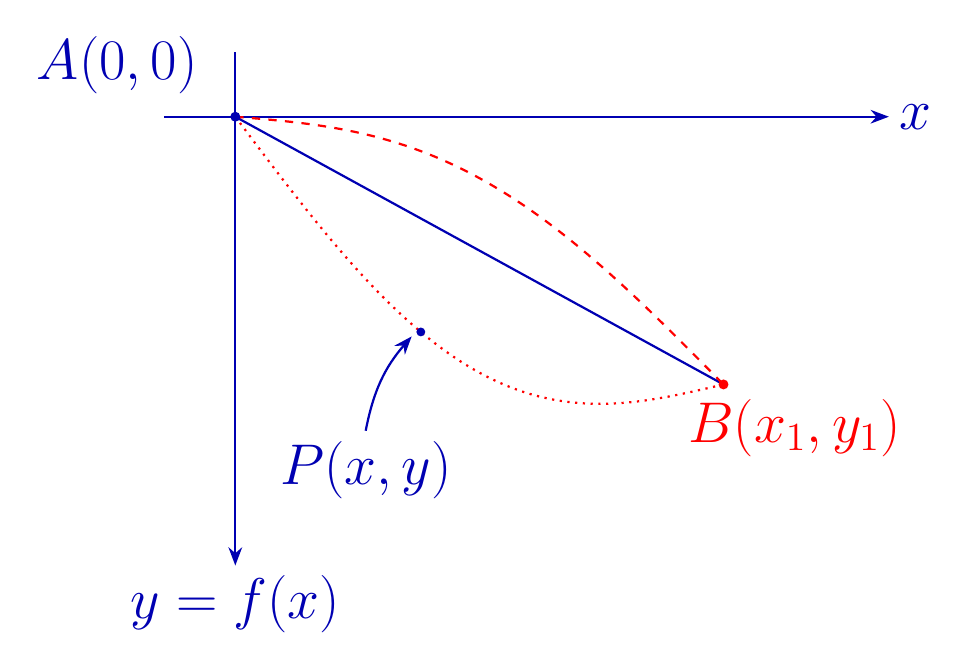
\begin{tikzpicture}[>=Stealth, thick, every node/.style={font=\fontsize{20}{24}\selectfont}]

  % ---- geometry ---------------------------------------------------------
  \def\Ax{0}   \def\Ay{0}
  \def\Bx{6.2} \def\By{-3.4}
  \def\ampOne{1.55}   % outer (lower) curve
  \def\ampTwo{1.15}   % inner (upper) curve

  % ---- axes ---------------------------------------------------------
  \draw[blue!70!black, ->] (-0.9,0) -- (8.3,0) node[right] {$x$};
  \draw[blue!70!black, ->] (0,0.82) -- (0,-5.7) node[below] {$y=f(x)$};

  \node[blue!70!black] at (-1.5,0.65) {$A(0,0)$};

  % ---- straight chord AB -------------------------------------------------
  \draw[blue!70!black] (\Ax,\Ay) -- (\Bx,\By);

  % ---- the family of curved paths, y(s) = linear(s) - amp*sin(pi s) --------
  \draw[red, dotted, samples=120, domain=\Ax:\Bx, variable=\x]
    plot ({\x}, {(\By)*(\x/\Bx) - \ampOne*sin(180*(\x/\Bx))});
  \draw[red, dashed, samples=120, domain=\Ax:\Bx, variable=\x]
    plot ({\x}, {(\By)*(\x/\Bx) + 0.8*\ampTwo*sin(180*(\x/\Bx))});

  \fill[blue!70!black] (\Ax,\Ay) circle (1.8pt);
  \fill[red] (\Bx,\By) circle (1.8pt);
  \node[red] at ($(\Bx,\By)+(0.9,-0.55)$) {$B(x_1,y_1)$};

  % ---- marked point P(x,y) on the outer curve -----------------------------
  \pgfmathsetmacro{\sP}{0.38}
  \pgfmathsetmacro{\xP}{\sP*\Bx}
  \pgfmathsetmacro{\yP}{(\By)*\sP - \ampOne*sin(180*\sP)}
  \fill[blue!70!black] (\xP,\yP) circle (1.6pt);
  \node[blue!70!black] at ($(\xP,\yP)+(-0.7,-1.75)$) (Plabel) {$P(x,y)$};
  \draw[blue!70!black, ->, thick] (Plabel.north) to[bend left=15] (2.24,-2.79);

\end{tikzpicture}
\end{document}
